\documentclass{beamer}
\usepackage{ctex}
\usepackage{tikz}
\usepackage{tikz-cd}

\usepackage{unicode-math}
%\setmathfont{STIX Two Math}
%\setmathfont{TeX Gyre Termes Math}
\setmathfont{Libertinus Math}
%\setmathfont{Fira Math}

\usepackage{graphicx} % Allows including images
\graphicspath{{./images/}}

%%%%%%%% FONT TIMESAVES %%%%%%%
\newcommand{\bT}{\mathbb{T}}
\newcommand{\bN}{\mathbb{N}}
\newcommand{\bI}{\mathbb{I}}

\newcommand{\cC}{\mathcal{C}}

%%%%%%%% CATEGORY THEORY %%%%%%%
\newcommand{\id}{\mathrm{id}}
\DeclareMathOperator{\Hom}{Hom}

\newcommand{\cat}[1]{\mathrm{#1}}
\newcommand{\Set}{\cat{Set}}

\DeclareFontFamily{U}{dmjhira}{}
\DeclareFontShape{U}{dmjhira}{m}{n}{ <-> dmjhira }{}

\DeclareRobustCommand{\yo}{\text{\usefont{U}{dmjhira}{m}{n}\symbol{"48}}}

\DeclareMathOperator*{\colim}{colim}

\newcommand{\inl}{\operatorname{inl}}
\newcommand{\inr}{\operatorname{inr}}

%%%%%%%%% GEOMTERY %%%%%%%%%%%%%%
\newcommand{\Spec}{\operatorname{Spec}}
\newcommand{\Zar}{\mathrm{Zar}}

%%%%%%%%% TYPE THEORY %%%%%%%%%%%
\newcommand{\OO}{\bigcirc}
\newcommand{\UU}{\mathcal{U}}
\newcommand{\isEquiv}{\bibopenparen{isEquiv}}
\newcommand{\hlevel}{\mathrm{hlevel}}
\newcommand{\isContr}{\operatorname{isContr}}
\newcommand{\isProp}{\operatorname{isProp}}
\newcommand{\Prop}{\mathrm{Prop}}
\newcommand{\Pos}{\mathrm{Pos}}
\newcommand{\DLat}{\mathrm{DLat}}
\newcommand{\refl}{\mathrm{refl}}
\newcommand{\isModal}{\operatorname{isModal}}
\newcommand{\ap}{\operatorname{ap}}
\newcommand{\fib}{\operatorname{fib}}
\newcommand{\im}{\operatorname{im}}
\newcommand{\tot}{\mathrm{tot}}
\newcommand{\pt}{\mathrm{pt}}

\title{Poset Type Theory 相关概念}

\date{}

\begin{document}

\begin{frame}
    % Print the title page as the first slide
    \titlepage
\end{frame}

\begin{frame}{dependent choice \cite{hottbook}}
$X$ 和 $Y$ 的一个\textbf{关系} $R$ 就是 $X \times Y$ 的一个子集 ($R \subseteq X\times Y$). 如果 $(a,b)\in R$, 我们也记为 $a\,R\,b$. $X$ 上的一个\textbf{齐次关系}就是 $R \subseteq X\times X$
\vspace{5mm}

$X$ 上的\textbf{齐次关系} $R$ 被称为\textbf{全关系}，如果对于每个 $a \in X$，
存在某个 $b \in X$ 使得 $a\,R\,b$ 成立。

\vspace{5mm}
\textbf{依赖选择公理}可以陈述如下：对于每个非空\textbf{集合} $X$ 和 $X$ 上的每个全关系 $R$，
存在 $X$ 中的一个\textbf{序列} $(x_n)_{n \in \mathbb{N}}$ 使得
\[
x_n\,R\,x_{n+1} \quad \text{对所有 } n \in \mathbb{N} \text{ 成立。}
\]
\end{frame}

\begin{frame}{$n$-type \cite{hottbook}}
对 $n \geq -2$，通过递归定义谓词 $\mathsf{is}\text{-}n\text{-}\mathsf{type} : \UU \to \UU$ 如下：
\[
\mathsf{is-}n\mathsf{-type}(X) :\equiv 
\begin{cases} 
\mathsf{isContr}(X) & \text{if } n = -2, \\
\prod_{(x,y:X)} \mathsf{is-}n'\mathsf{-type}(x =_X y) & \text{if } n = n' + 1.
\end{cases}
\]

\vspace{1em}

如果 $\mathsf{is}\text{-}n\text{-}\mathsf{type}(X)$ 是被占据的（inhabited），
则我们说 $X$ 是一个 \textbf{$n$-类型}，或有时称它是 \textbf{$n$-截断的}。
\end{frame}

\begin{frame}{Whitehead's principle \cite{hottbook}}
设 $A$ 和 $B$ 是 $n$-类型，且 $f : A \to B$ 满足
\begin{enumerate}
    \item[(i)] $\|f\|_0 : \|A\|_0 \to \|B\|_0$ 是一个\textbf{双射}，且
    \item[(ii)] $\pi_k(f) : \pi_k(A, x) \to \pi_k(B, f(x))$ 对所有 $k \geq 1$ 及所有 $x : A$ 是一个\textbf{双射}。
\end{enumerate}
则 $f$ 是一个\textbf{等价}。

\vspace{5mm}
一个映射 $f$，若 $\|f\|_0$ 是双射且对所有 $k$，$\pi_k(f)$ 是双射，
则称为 \textbf{$\infty$-连通的} 或 \textbf{弱等价}。
这等价于要求 $f$ 对所有 $n$ 都是 $n$-连通的。
一个类型 $Z$ 称为 \textbf{$\infty$-截断的} 或 \textbf{超完备的}，
如果诱导映射
\[
(- \circ f) : (B \to Z) \to (A \to Z)
\]
在 $f$ 为 $\infty$-连通时是一个等价——也就是说，
如果 $Z$ 认为每个 $\infty$-连通映射都是等价。
那么，如果我们想把 \textbf{Whitehead 原理} 作为公理来假设，
我们可以使用以下两种等价形式中的任意一种。

\begin{itemize}
    \item 每个 $\infty$-连通函数都是等价。
    \item 每个类型都是 $\infty$-截断的。
\end{itemize}
\end{frame}

\begin{frame}{finite non-empty posets(有限非空偏序集)}
集合 $P$ 上有一个自反、反对称、传递的关系 $≤$，且元素个数有限。
\end{frame}

\begin{frame}{finite, bounded, non-degenerate distributive lattices(有限有界非退化分配格)}
  \begin{itemize}
  \item 格：任意两个元素有最小上界 $∨$（并）和最大下界 $∧$（交）

  \item 分配律：$x∧(y∨z)=(x∧y)∨(x∧z)$ 以及其对偶

  \item 有界：存在最大元 $⊤$ 和最小元 $⊥$

  \item 非退化：$⊥≠⊤$（至少两个元素）
\end{itemize}
\end{frame}

\begin{frame}[fragile,shrink]{有限呈现分配格（finitely presented distributive lattice）}
\begin{figure}[htbp]
\centering
%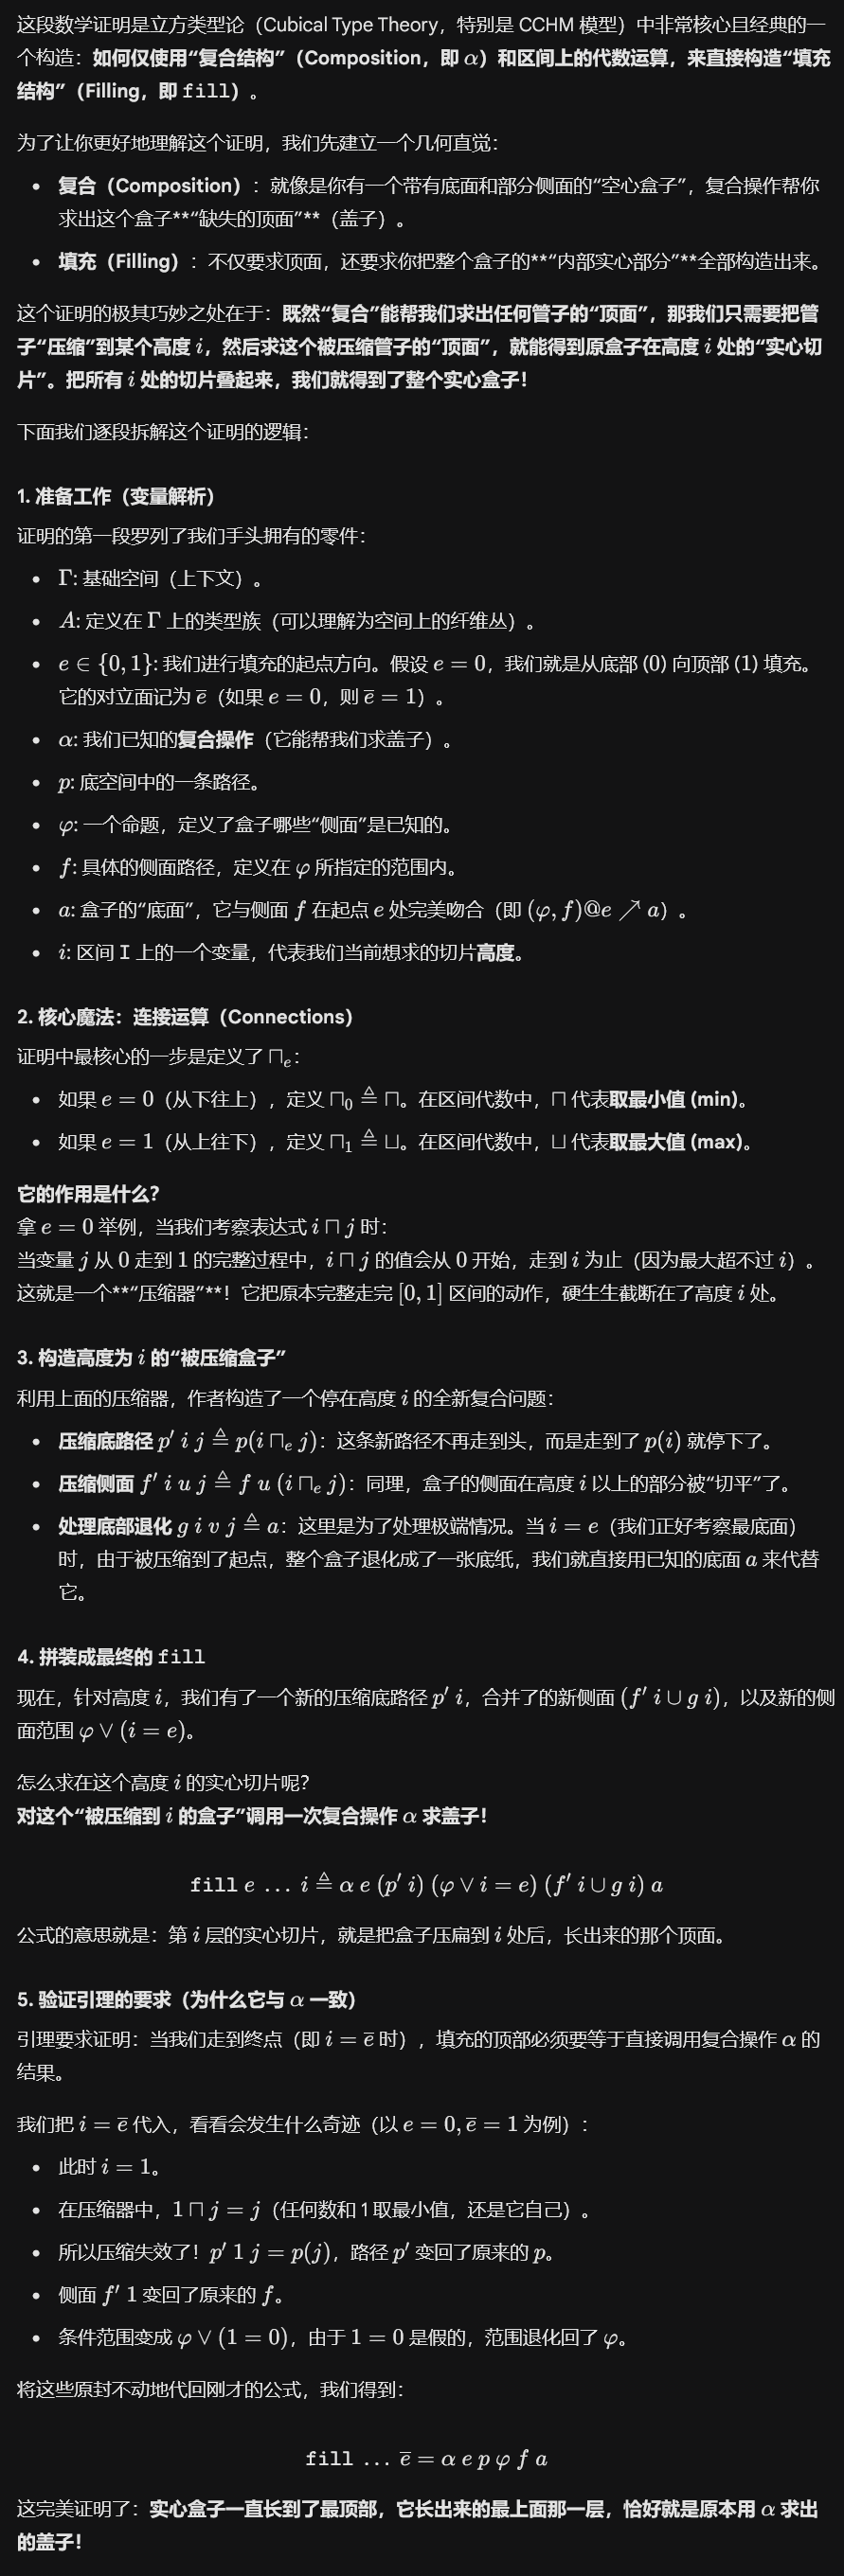
\includegraphics[width=0.75\textwidth]{comp_fill}
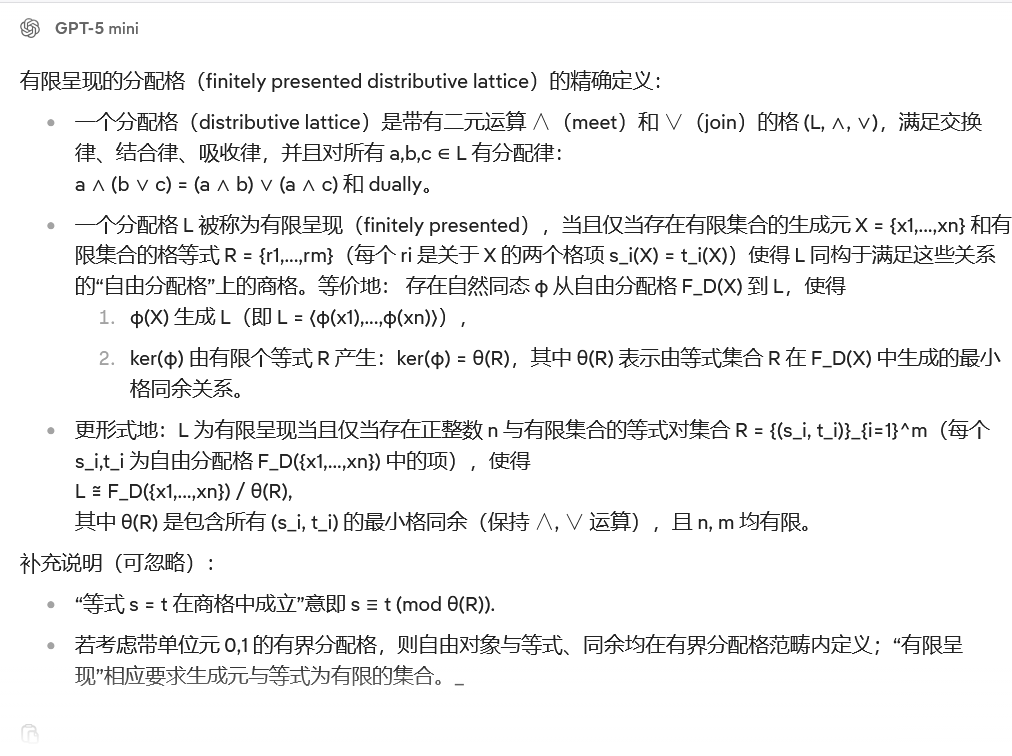
\includegraphics[width=\textwidth]{finitely_presented_distributive_lattice}
\end{figure}
\end{frame}

\begin{frame}{子偏序集（Subposet）}
A poset $P^* = (X^*, \le^*)$ is called a \textbf{subposet} of another poset $P = (X, \le)$ provided that $X^*$ is a subset of $X$ and $\le^*$ is a subset of $\le$. The latter condition is equivalent to the requirement that for any $x$ and $y$ in $X^*$ (and thus also in $X$), if $x \le^* y$ then $x \le y$.
\end{frame}

\begin{frame}{偏序集（Poset）中的 Embedding}
设 \((P, \le_P)\) 和 \((Q, \le_Q)\) 是两个偏序集。一个映射 \(f: P \to Q\) 称为 \textbf{嵌入}（order embedding），如果它满足：
\[
\forall x, y \in P,\quad x \le_P y \ \iff\ f(x) \le_Q f(y).
\]
即 \(f\) 既是\textbf{序保持}（\(x \le y \Rightarrow f(x) \le f(y)\)），又是\textbf{序反射}（\(f(x) \le f(y) \Rightarrow x \le y\)），且由此可推出 \(f\) 一定是\textbf{单射}（因为若 \(f(x)=f(y)\)，则由 \(f(x)\le f(y)\) 和 \(f(y)\le f(x)\) 得 \(x\le y\) 且 \(y\le x\)，故 \(x=y\)）。

- 嵌入的像 \(f(P)\) 是 \(Q\) 的一个子偏序集，且 \(f\) 给出了 \(P\) 与 \(f(P)\) 之间的\textbf{同构}（因为 \(f\) 是双射到像且保持/反射序）。
- 因此，\textbf{嵌入本质上等价于子偏序集}：每个子偏序集对应一个包含映射（它是嵌入）；反之，每个嵌入的像就是一个子偏序集。
\end{frame}

\begin{frame}[fragile,shrink]{偏序集的 lower set \cite{lower_set}}
每个有限分配格同构于某个有限偏序集的下集格（lower set lattice）

Let $(X, \leq)$ be a \textbf{preordered set} (the same as a partially ordered set except the requirement $x \leq y$, $y \leq x$ implying $x = y$ is dropped).

An \textbf{upper set} in $X$ (also called an \emph{upward closed set}, \emph{up set}, \emph{increasing set}, or an \emph{isotone set}) is a subset $U$ that is ``closed under going up'', in the following sense: for all $u$ in $U$ and $x$ in $X$, if $u \leq x$, then $x$ is in $U$.

The \textbf{dual} notion is a \textbf{lower set} (also called a \emph{downward closed set}, \emph{down set}, \emph{decreasing set}, or a \emph{semi-ideal}), which is a subset $L$ that is ``closed under going down'': for all $l$ in $L$ and all $x$ in $X$, if $x \leq l$, then $x$ is in $L$.

The term \textbf{order ideal} is sometimes used as a synonym for a lower set. However, an \textbf{ideal} is also commonly defined specifically as a lower set which is \textbf{upward directed}. Dually, a \textbf{filter} is an upper set that is directed downward (that is, every finite subset has a lower bound).

For a \textbf{well-ordered set}, a lower set is usually called an \textbf{initial segment}.
\end{frame}

\begin{frame}
给定有限偏序集 $P$, 考虑它的所有\textbf{lower sets}
\begin{itemize}
    \item 下集对并和交封闭, 且包含 $\emptyset$ 和 $P$, 构成一个分配格, 记作 $\mathcal{O}(P)$
    \item 这个格同构于 $\Pos(P,[1])$, 因为每个单调映射 $f : P\to \{0,1\}$ 对应下集 $f^{-1}(0)$. ($\Pos(-,[1]) : \Pos \to \DLat$ 是一个反变函子)
\end{itemize}
\end{frame}

\begin{frame}{join-irreducible elements(并·不可约元)}
In a lattice, an element $x$ is join-irreducible if $x$ is not the join of a finite set of other elements. Equivalently, $x$ is join-irreducible if it is neither the bottom element of the lattice (the join of zero elements) nor the join of any two smaller elements.

\vspace{5mm}
An element $a$ in a lattice $L$ is said to be join irreducible iff $a$ is not a bottom element, and, whenever $a=b∨c$, then $a=b$ or $a=c$. 

\vspace{5mm}
 An element $x$ is join-prime if it differs from the bottom element, and whenever $x ≤ y ∨ z$, either $x ≤ y$ or $x ≤ z$.
\end{frame}

\begin{frame}{从格运算定义偏序}
给定一个格 $(L, ∧, ∨)$，可以按下列自然方式从格运算定义偏序 $≤$：

\vspace{5mm}
\begin{quote}
    对任意 $a,b ∈ L$，令 $a ≤ b$ 当且仅当 $a ∧ b = a$. 等价地也可用 $a ∨ b = b$。
\end{quote} 
\end{frame}

\begin{frame}{从分配格到偏序集}
给定有限有界分配格 $L$，取 $L$ 的所有 join-irreducible elements
\begin{itemize} 
    \item 按自然序构成一个偏序集 $J(L)$
    \item $J(L)$ 恰好同构于 $\DLat(L,[1])$ 说明见下页. ($\DLat(-,[1]) : \DLat \to \Pos$ 是一个反变函子)
\end{itemize}

\vspace{5mm}
$\Pos(-,[1]) : \Pos \to \DLat$ 和 $\DLat(-,[1]): \DLat \to \Pos$ 这两个反变函子是伴随等价(adjoint equivalence)
\end{frame}

\begin{frame}[fragile,shrink]
\begin{figure}[htbp]
\centering
%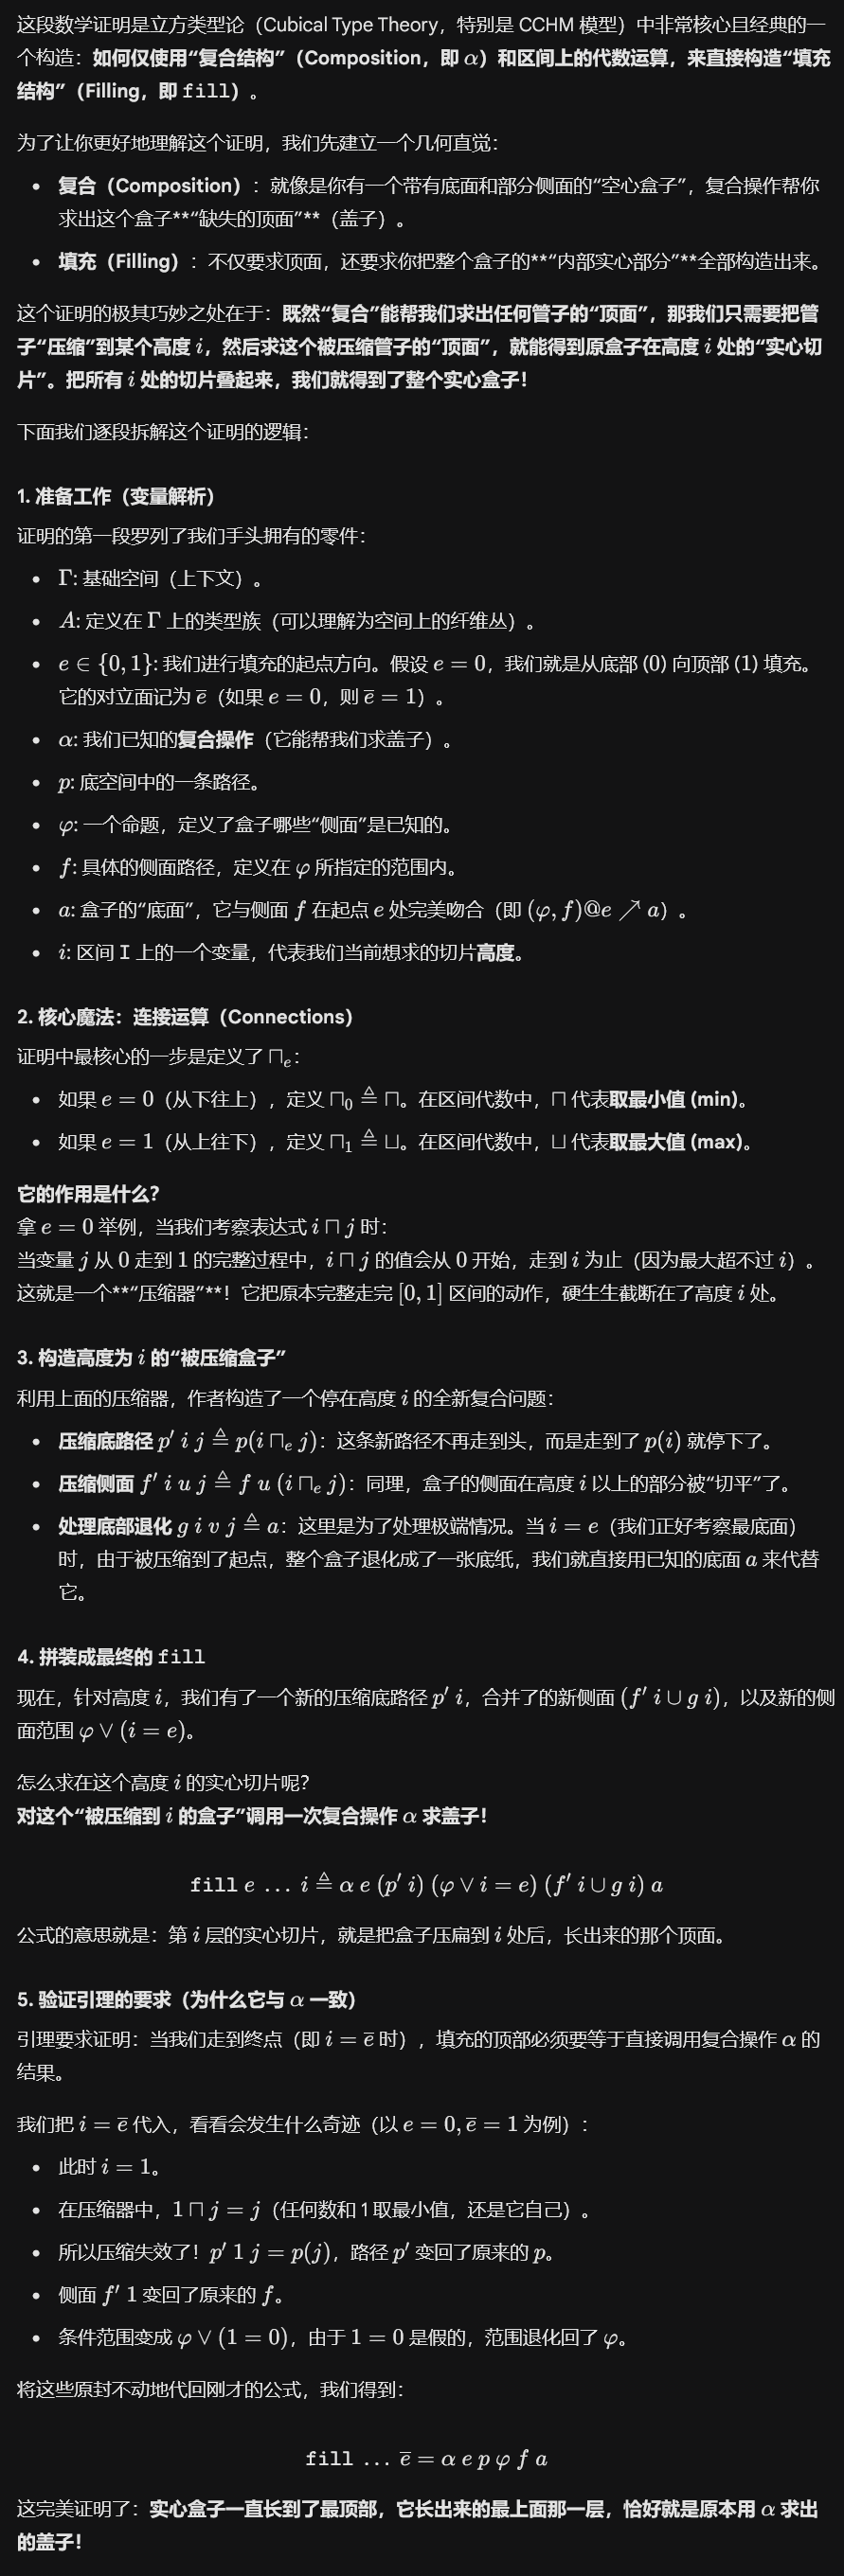
\includegraphics[width=0.75\textwidth]{comp_fill}
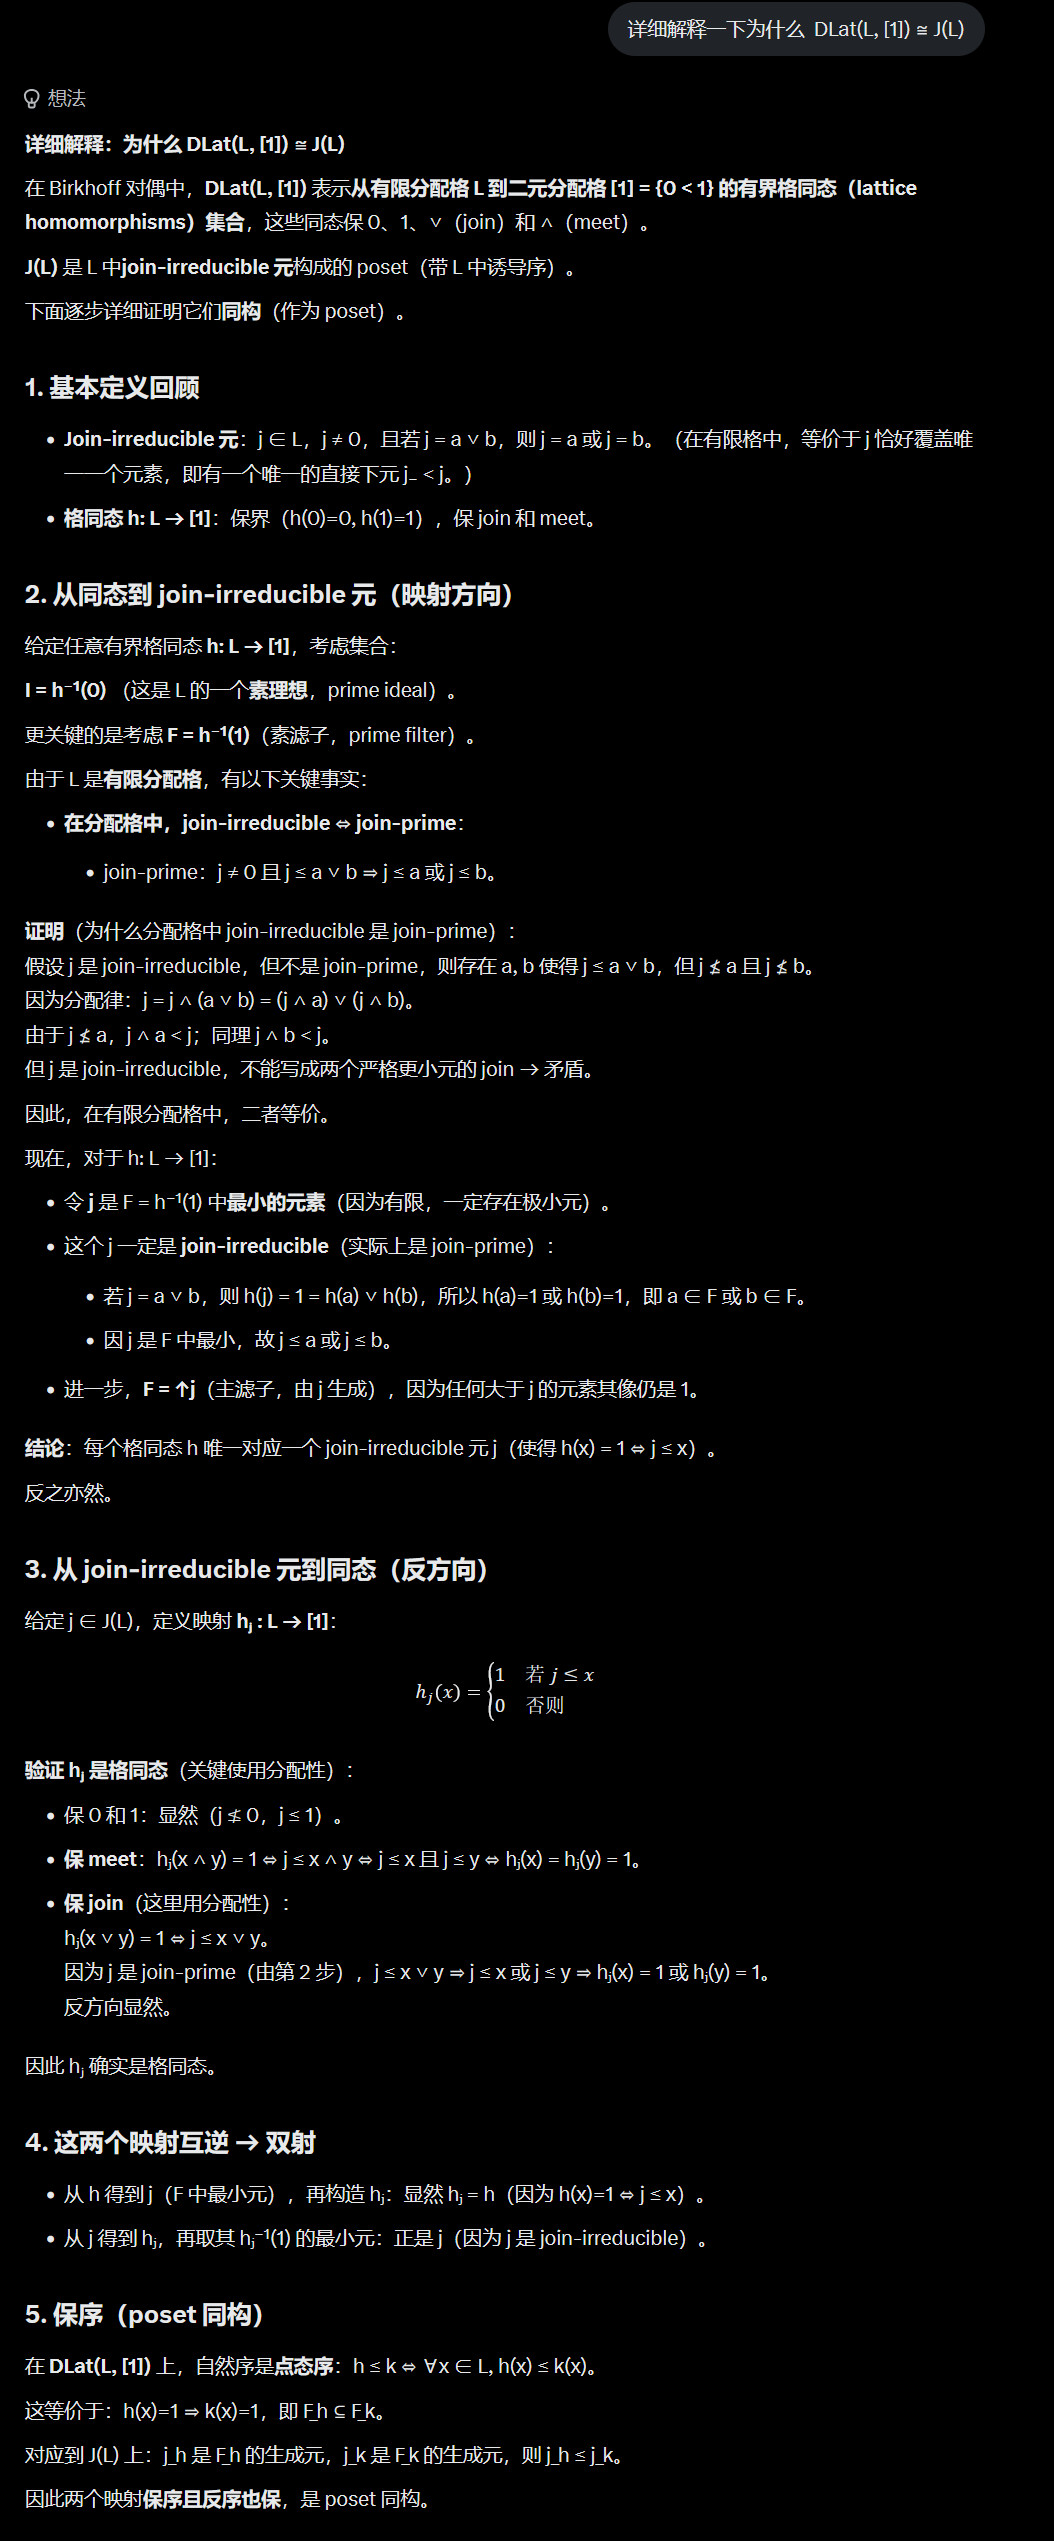
\includegraphics{DLat_J}
\end{figure}
\end{frame}

\begin{frame}
总的思路是把有限非空偏序集通过 Birkhoff duality 转换为有限有界非退化分配格, 又因为有限分配格又可以用有限呈现分配格表示, 下面讨论怎么取 cofibration 的问题, 就可以化为有限呈现分配格的问题.

\vspace{5mm}
而且, 对于有限分配格 $L$, 根据上面的构造, $L \cong \mathcal{O}(J(L))$. $\mathcal{O}(J(L))$ 是幂集 $\mathcal{P}(J(L))$ 的一个子格. 而 $\mathcal{P}(J(L))$ 是一个 \textbf{boolean lattice(布尔格)}. 这样就把一个有限分配格嵌入了一个布尔格, 相关问题可以转化为\textbf{boolean SAT}问题.
\end{frame}

\begin{frame}[fragile,shrink]{The cofibration classifier $Φ$}
\begin{itemize}
    \item base category of cubes $\Box$ is given by finite non-empty poset
    \item 在范畴 $\Box$ 中, $X$ 上的一个 sieve $S$ 是一族进入 $X$ 的态射, 满足对任意 $f : Y \to X \in S$, 任意 $g : Z \to Y$, 我们有 $f \circ g \in S$.
    \item 由单个 morphism 生成的 sieve：记作 $\langle f \rangle$，其中 $f: Y \to X$。它包含所有能通过 $f$ 分解的态射
    \[
    \begin{tikzcd}
      & Y \arrow[dr,"f"] & \\
    Z \arrow[ur] \arrow[rr] & & X
    \end{tikzcd}
    \]
    \item The cofibration classifier $Φ$ is constructed at some stage $X$ by starting with the meet-semilattice of sieves on $X$ generated by embeddings, and freely adding joins. 下一页解释
\end{itemize}
\end{frame}

\begin{frame}[fragile,shrink]
\begin{itemize}
  \item 先找出所有由 embeddings 生成的 sieves：即 $\{ \langle e \rangle \mid e \text{ 是一个 embedding} \}$
  \item 然后取这些 sieves 生成的最小的 meet-semilattice:
    \begin{itemize}
        \item 包含所有这些 $  \langle e \rangle  $
        \item 对任意有限个这样的 sieves，取它们的交（meet），仍然留在里面. $\langle e_1\rangle \land \langle e_2\rangle := \langle e_1\rangle \cap \langle e_2\rangle$, 得到的确实是一个 sieve, 但是不是由某一个嵌入生成的呢? 目前看, 只有空集的情况除外, 其他情况确实如此.
        \item 包含顶元素（全 sieve）, 就是 $\langle id\rangle$
    \end{itemize}
    这步得到的是一个只有 meets（交运算）、没有 joins（并运算） 的结构 —— 即 meet-semilattice。它只包含“由子 poset 生成的基本 cofibrations 以及它们的交”。
  \item 在上面得到的 meet-semilattice 上，自由地添加 joins（并运算）
    \begin{itemize}
        \item “自由”意思是：我们形式化地往里加入所有可能的有限并（joins），并保持分配律等必要性质，但不额外加入其他关系
    \end{itemize}
\end{itemize}

\vspace{5mm}
$\Phi(X)$ 就是上面得到的分配格
\end{frame}

\begin{frame}
$\Phi(X)$ 是 $X$ 上的所有 decidable sieves 的一个真子集.

\vspace{5mm}
由 $\{0,1\} \hookrightarrow \{0 < 1\}$ 生成的 sieve 不属于 $\Phi(\{0 < 1\})$. 因为 $\{0,1\}\hookrightarrow\{0 < 1\}$ 不是一个嵌入(embedding). 
\end{frame}

% 参考文献帧，长列表自动分页
\begin{frame}[allowframebreaks]{参考文献}
\begin{thebibliography}{99}

\bibitem{hottbook}
Homotopy Type Theory: Univalent Foundations of Mathematics.

\bibitem{lower_set}
Upper and lower sets. \url{https://en.wikipedia.org/wiki/Upper_and_lower_sets}.

\end{thebibliography}
\end{frame}

\end{document}